%%%%%%%%%%%%%%%%%%%%%%
%% APPENDIX FIGURES %%
%%%%%%%%%%%%%%%%%%%%%%
\begin{figure}[H]
\caption{Road Program Completion Dates}
\label{fig:pmgsy_dates}
\begin{center}
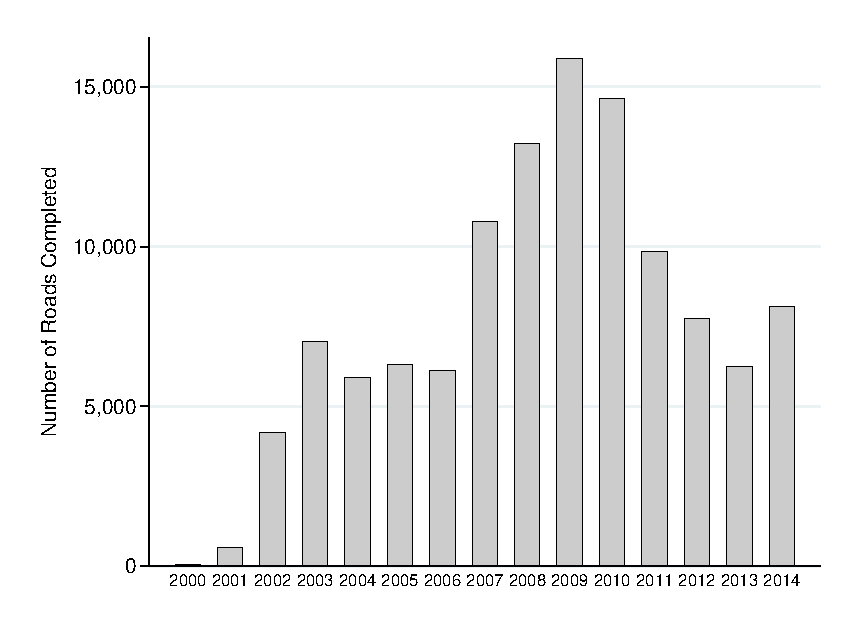
\includegraphics[scale=0.77]{\filepath/pmgsy_dates}  \\
\end{center}
\newline
\footnotesize{The figure shows the number of roads completed under the
  PMGSY road construction program, by year.}
\end{figure}

\begin{landscape}
  \begin{figure}[H]
    \caption{Forest Cover in 2000 According to Different Remote Sensing Sources}
    \label{fig:gfc_ndvi}
      \setlength{\fboxsep}{0pt}
      \setlength{\fboxrule}{1pt}
      \setlength\tabcolsep{0pt}
    \begin{tabular}{ccc}
      Vegetation Continuous Fields & Global Forest Cover & NDVI \\
      \fbox{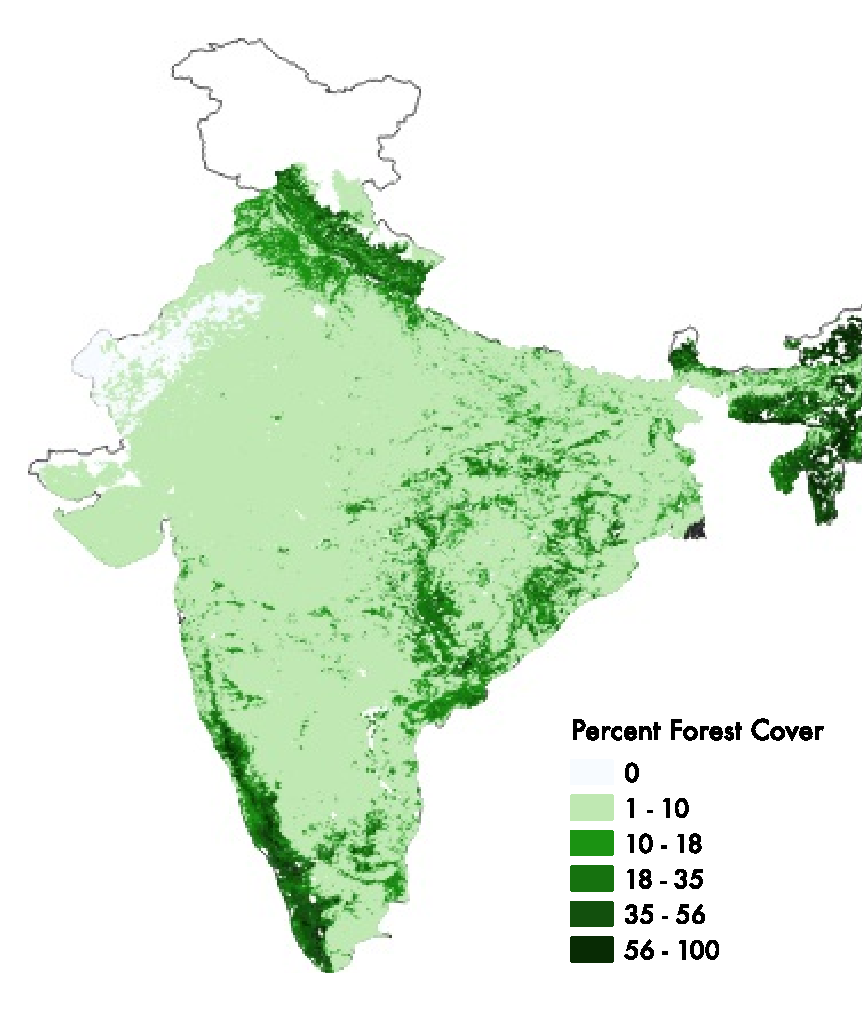
\includegraphics[scale=0.55]{\filepath/compare_vcf}} &
      \fbox{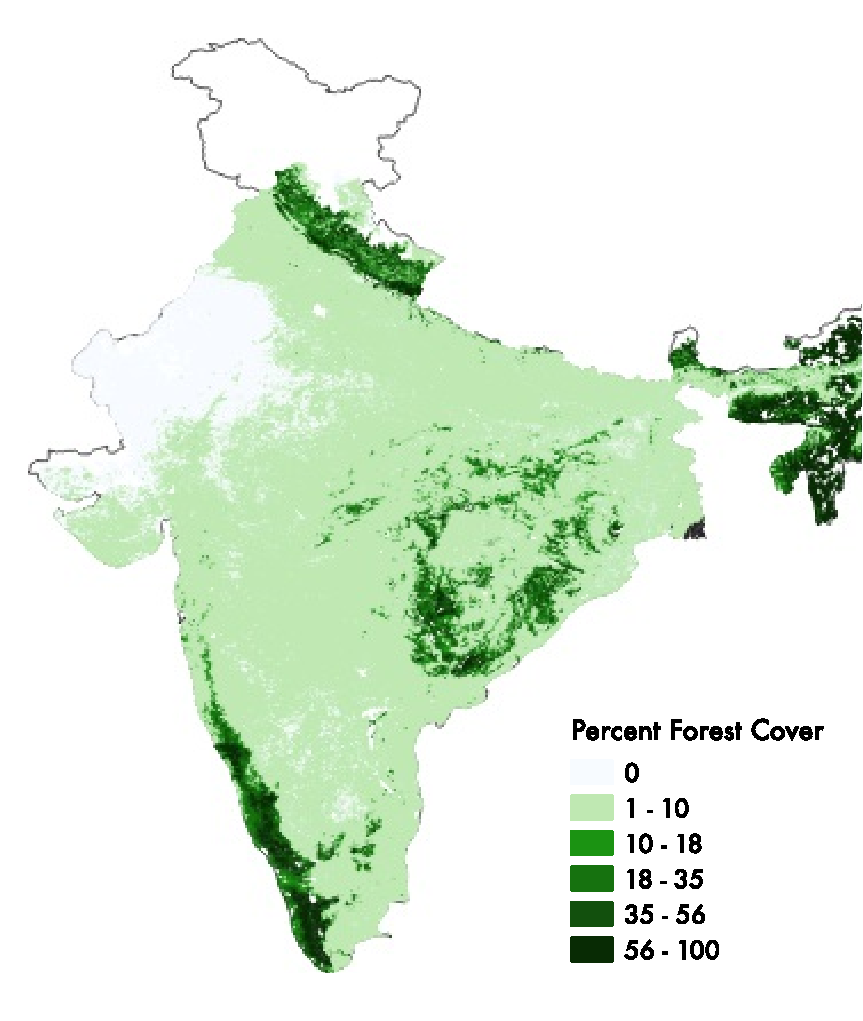
\includegraphics[scale=0.55]{\filepath/compare_gfc}} &
      \fbox{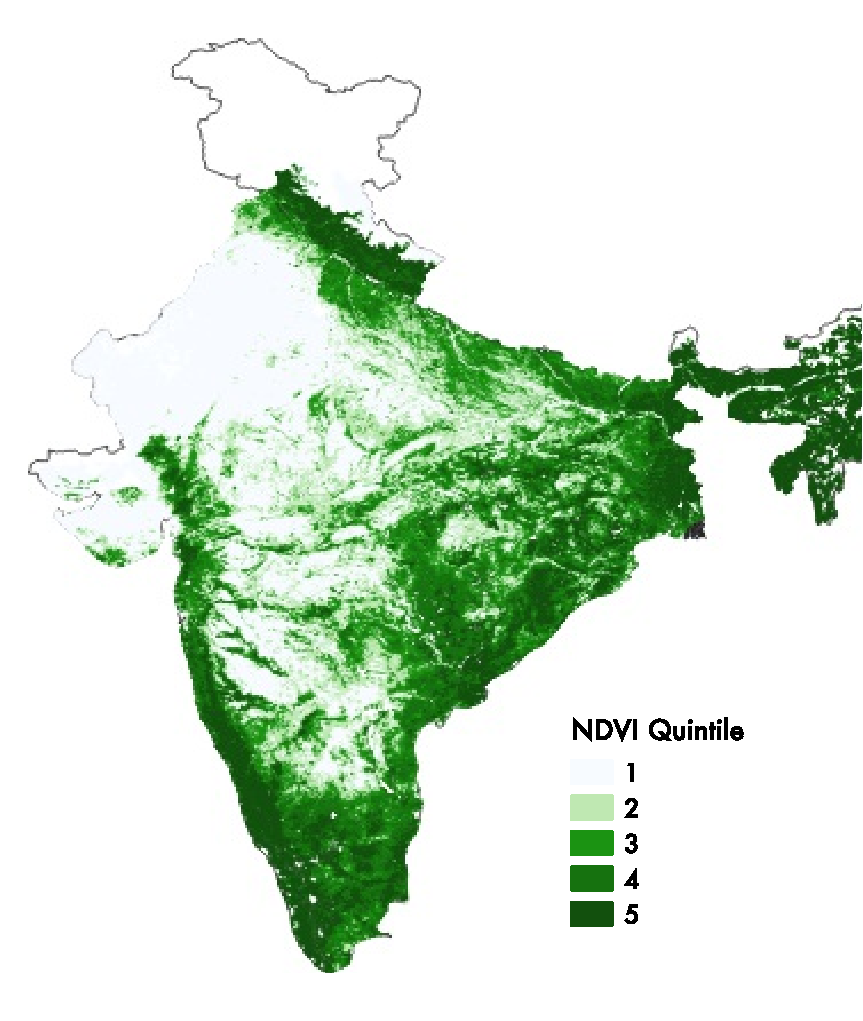
\includegraphics[scale=0.55]{\filepath/compare_ndvi}} \\
      \setlength\tabcolsep{6pt}
    \end{tabular}
    \newline \footnotesize{The figure compares three different remote
      sensing measures of forest cover in India for the year
      2000. Gridded forest cover data are aggregated to village and
      town polygons according to the 2011 population
      census. Vegetation Continuous Fields and Global Forest Cover can
      be directly interpreted as the average share of land covered by
      forest in the year 2000. For NDVI, we report quintiles of the
      NDVI index measured in February of 2000, the time of year when
      forest is most distinguishable from crop cover \cite{FR03}.}
  \end{figure}
\end{landscape}

\begin{figure}[H]
\caption{Regression Discontinuity Balance Tests}
\label{fig:rd_balance}
\begin{center}
\includegraphics[scale=0.5]{\filepath/rd_baseline_graphs}  \\
\end{center}
\newline
\footnotesize{The figure displays a graphical form of the regression
  discontinuity balance test. Each graph shows the means of a variable
  measured at baseline in bins defined by population relative to the
  rural road program treatment threshold. The linear fits and standard
  errors are estimated from Equation~\ref{eq:rd1}. The vertical line
  shows the treatment threshold; the jump in the fit at this line is
  the regression discontinuity treatment estimate. The dependent
  variable in each panel (left-to-right, top-to-bottom) is (A) log
  forest cover in 2000; (B) average forest cover in 2000; (C) change
  in log forest cover from 2000 to 2005; (D) the share of households
  whose primary cooking fuel is firewood; (E) the log of night light
  luminosity in 2000; and (F) average night light luminosity in
  2000. In Panel C, we omit villages with roads built before 2006, to
  ensure that balance estimates are not contaminated by the small
  number of treated villages before this date. All estimates include
  district-population threshold fixed effects.}
\end{figure}

\begin{figure}[H]
\caption{Regression Discontinuity Density Test}
\label{fig:rd_mccrary}
\begin{center}
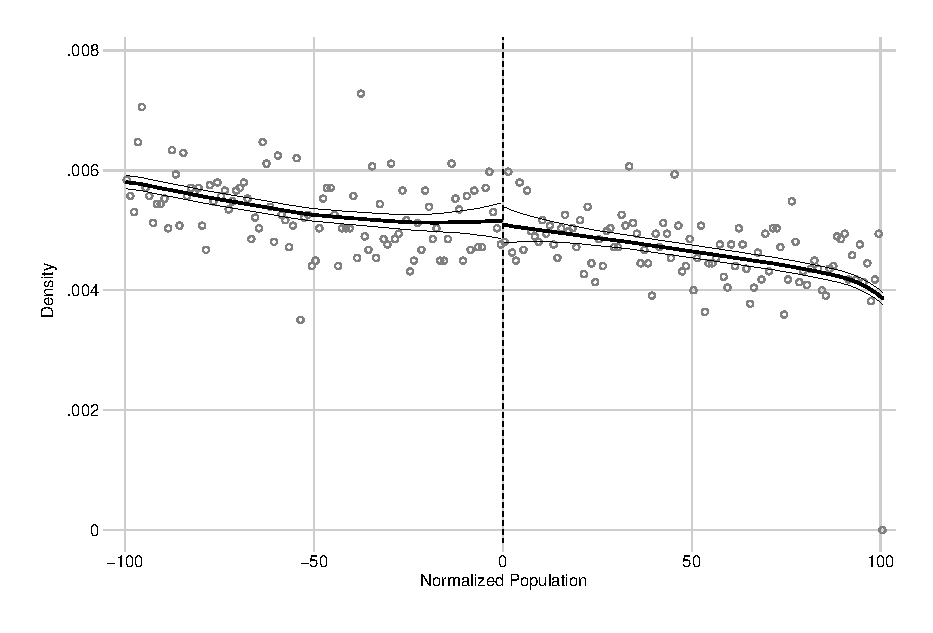
\includegraphics[scale=1]{\filepath/deforest_mccrary}  \\
\end{center}
\newline
\footnotesize{The figure displays a graph from a regression
  discontinuity density test \cite{MC08}. The X axis shows the
  population relative to the road program treatment eligibility
  threshold. The Y axis shows a kernel estimate of the density of
  villages in a given normalized population band. The lines display
  non-parametric fits to the density function along with 95\%
  confidence intervals.}
\end{figure}

\begin{figure}[H]
\caption{Difference-in-Differences Estimates of Impact of
    \cnewline Rural Roads on Forest Cover (Long Panel)}
\label{fig:panel_4}
\begin{center}
\begin{tabular}{c}
Full Sample \\
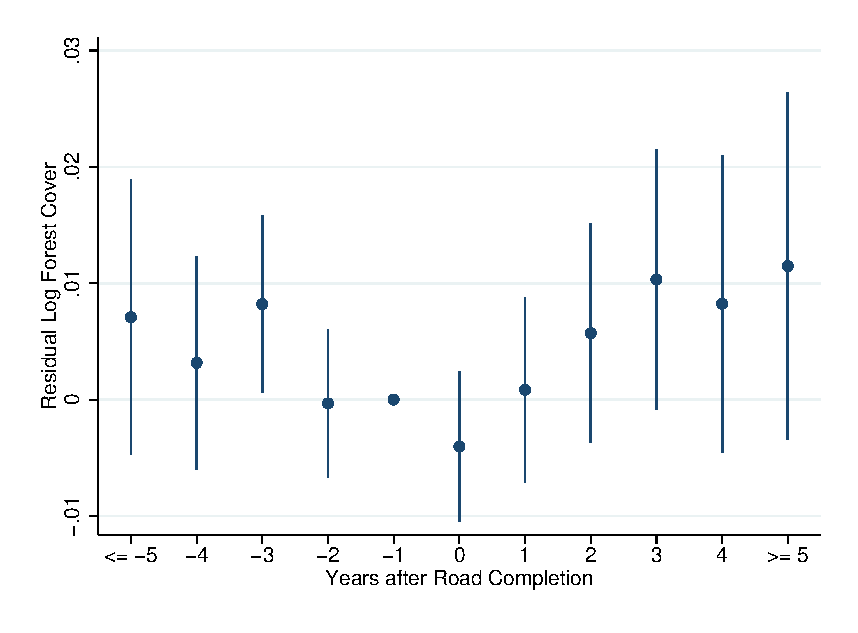
\includegraphics[scale=0.77]{\filepath/coefplot_bal_comp_5}  \\
\newline \newline \\
High Baseline Forest \\
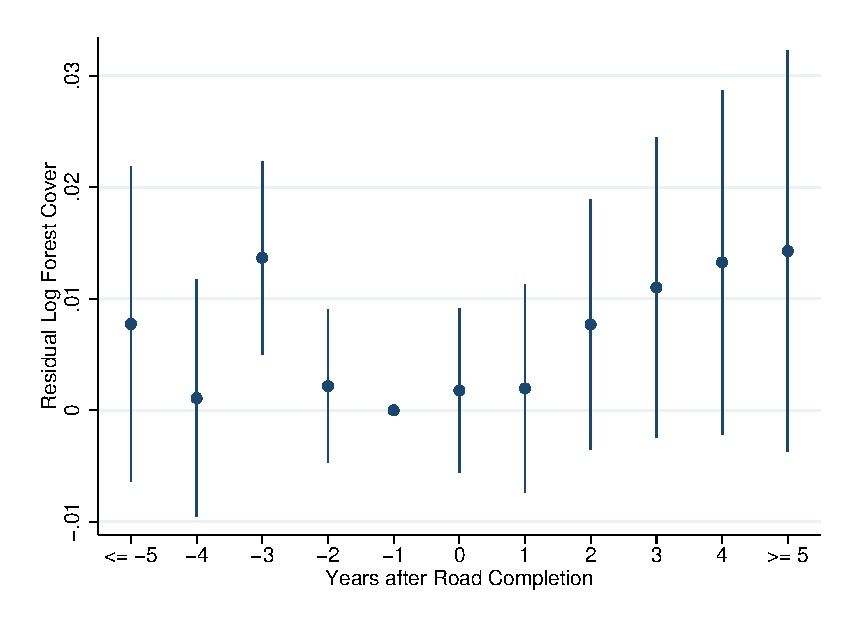
\includegraphics[scale=0.77]{\filepath/coefplot_bal_comp_5_thick}  \\
\newline
\end{tabular}
\end{center}
\newline
\footnotesize{The figure shows year-by-year estimates of log forest
  cover in villages that received new roads between 2001 and 2013. The
  figure is identical to Figure~\ref{fig:panel}, but with an
  additional estimate for the 5th year before and after
  treatment.  Villages are grouped on the X axis according to the year
  relative to road completion. Each point thus shows the average value
  of log forest cover in villages in a given year relative to the
  treatment year, controlling for village fixed effects, district*year
  fixed effects and baseline population * year and baseline log forest
  cover * year interactions. Standard errors are clustered at the
  village level.}
\end{figure}

%%%%%%%%%%%%%%%%%%%%%
%% APPENDIX TABLES %%
%%%%%%%%%%%%%%%%%%%%%

%% OLS: ROADS AND FOREST COVER
\begin{table}[H]
\begin{center}
\caption{OLS Regressions of Forest Cover on Rural Road Indicators}
\newcommand{\tablenote}{The table shows estimates from OLS regressions of
  village-level log forest cover in 2001 on an indicator variable that
  takes the value one if a village has a paved road in 2001. Column 1
  presents the bivariate estimates, and Columns 2 through 5 present
  estimates with progressively greater numbers of controls and fixed
  effects. Forest cover is calculated from Vegetation Continuous
  Fields. Population is measured in millions of people.}
\setlength{\linewidth}{.1cm} \begin{center}
\newcommand{\contents}{\begin{tabular}{l*{5}{c}}
\hline\hline
                    &         (1)   &         (2)   &         (3)   &         (4)   &         (5)   \\
\hline
Paved Road in 2001  &      -0.162***&      -0.270***&      -0.041***&      -0.025***&      -0.018** \\
                    &     (0.010)   &     (0.010)   &     (0.009)   &     (0.009)   &     (0.009)   \\
Population          &               &       0.476***&       0.862***&       0.896***&       0.910***\\
                    &               &     (0.013)   &     (0.012)   &     (0.012)   &     (0.012)   \\
Population\superscript{2}&               &      -0.037***&      -0.085***&      -0.092***&      -0.095***\\
                    &               &     (0.004)   &     (0.003)   &     (0.003)   &     (0.003)   \\
Distance in km to town of 10,000&               &               &               &               &       0.007***\\
                    &               &               &               &               &     (0.000)   \\
Distance in km to town of 100,000&               &               &               &               &      -0.000   \\
                    &               &               &               &               &     (0.000)   \\
Constant            &       3.405***&       3.083***&       2.786***&       2.764***&       2.533***\\
                    &     (0.004)   &     (0.008)   &     (0.007)   &     (0.007)   &     (0.013)   \\
\hline Fixed Effects              & None & None & State & State & District \\ 
N                   &      270871   &      270871   &      270871   &      270871   &      270871   \\
r2                  &        0.00   &        0.02   &        0.19   &        0.28   &        0.28   \\
\hline
\multicolumn{6}{p{\linewidth}}{$^{*}p<0.10, ^{**}p<0.05, ^{***}p<0.01$} \\
\multicolumn{6}{p{\linewidth}}{\footnotesize \tablenote}
\end{tabular} }
\setbox0=\hbox{\contents}
\setlength{\linewidth}{\wd0-2\tabcolsep-.25em} \contents \end{center}

\label{tab:ols}
\end{center}
\end{table}

%% RD: BALANCE TESTS
\begin{table}[H]
\begin{center}
  \caption{Regression Discontinuity Balance Tests}
  \label{tab:rd_balance}
\begin{tabular}{l r r r}\hline\hline Variable & RD Estimate  & N \\ \hline
Log Forest (2000) & -0.012 & 22365 \\ 
 & (0.027) & \\
Average Forest (2000) & -0.093 & 22365 \\ 
 & (0.101) & \\
Share Cooking with Firewood & -0.001 & 22317 \\ 
 & (0.003) & \\
Log Forest Change (2000-2005) & 0.012 & 22365 \\ 
 & (0.012) & \\
Mean Night Light (2000) & -0.019 & 21542 \\ 
 & (0.060) & \\
Log Night Light (2000) & -0.032 & 21542 \\ 
 & (0.029) & \\
\hline\hline \multicolumn{2}{p{24em}}{$^{*}p<0.10, ^{**}p<0.05,^{***}p<0.01$} \\ \end{tabular} 

\end{center}
\newline
\footnotesize{The table shows
  estimates from a regression discontinuity balance test. We run the
  regression discontinuity specification defined by
  Equation~\ref{eq:rd1} on variables measured before any rural road
  construction took place, and report the reduced form treatment
  estimates. Row 4 (Log Forest Change 2000-2005) tests for pretrends
  in forest cover; we exclude villages with roads built before 2006
  for this sample. All estimates include district-population threshold
  fixed effects.}
\end{table}

%% MORE RD HETEROGENEITY TABLE FOR REFEREES
\begin{table}[H]
\caption{Regression Discontinuity Estimates of Impact of \cnewline
  Rural Roads on Forest Cover (Heterogeneity Tests)}
\newcommand{\tablenote}{ The table shows reduced form regression
  discontinuity estimates of the impact of rural roads on forest
  cover. The specifications are comparable to those in Columns 2 and 3
  of Table~\ref{tab:rd} but for subsamples related to treatment
  heterogeneity of interest.  Columns 1 and 2 respectively show
  estimates for villages with above and below median distance to the
  nearest town of 100,000 or higher. Columns 3 and 4 respectively show
  estimates for villages with above and below median market
  access. Market access is measured with a trade elasticity of 8, the
  value suggested in \citeasnoun{DH12}; results are similar
  under other elasticities. Columns 5 and 6 restrict the sample
  respectively to villages with above median employment in logging and
  employment in wood-using industries. The outcome variable is log
  forest cover in 2013. All estimates include district-population
  threshold fixed effects and a control for baseline forest cover.}
\setlength{\linewidth}{.1cm} \begin{center}
\newcommand{\contents}{\begin{tabular}{l*{6}{c}}
\hline\hline
 & \multicolumn{2}{c}{\underline{Dist. to Town}} & \multicolumn{2}{c}{\underline{Market Access}} & \underline{Logging} & \underline{Ind. Wood Use} \\ 
%PYTHON_HEADER
                    &         Low   &        High   &         Low   &        High   &        High   &        High   \\
\hline
Above Population Threshold&      -0.008   &       0.005   &      -0.001   &      -0.001   &      -0.002   &       0.021   \\
                    &     (0.019)   &     (0.022)   &     (0.023)   &     (0.021)   &     (0.015)   &     (0.020)   \\
\hline
N                   &       11180   &       11166   &       10076   &       10074   &       22365   &       11283   \\
r2                  &        0.82   &        0.81   &        0.81   &        0.81   &        0.81   &        0.81   \\
\hline
\multicolumn{7}{p{\linewidth}}{$^{*}p<0.10, ^{**}p<0.05, ^{***}p<0.01$} \\
\multicolumn{7}{p{\linewidth}}{\footnotesize \tablenote}
\end{tabular} }
\setbox0=\hbox{\contents}
\setlength{\linewidth}{\wd0-2\tabcolsep-.25em} \contents \end{center}

\label{tab:rd_het}
\end{table}

%% RD: ALTERNATE BANDWIDTHS
\begin{landscape}
\begin{table}[H]
\caption{Regression Discontinuity Estimates of Impact of
    \cnewline Rural Roads on Forest Cover (Alternate Bandwidths)} \newcommand{\tablenote}{
  The table shows reduced form regression discontinuity estimates of
  the impact of rural roads on forest cover. The specifications are
  comparable to those in Columns 2 and 3 of Table~\ref{tab:rd} but
  with alternate bandwidths defined in the bandwidth row of the
  table. The outcome variable is log
  forest cover in 2013. All estimates include district-population threshold
  fixed effects and a control for baseline forest cover.} \setlength{\linewidth}{.1cm} \begin{center}
\newcommand{\contents}{\begin{tabular}{l*{8}{c}}
\hline\hline
 & \multicolumn{4}{c}{\underline{Log Forest (2013)}} & \multicolumn{4}{c}{\underline{Average Forest (2013)}} \\ 
%PYTHON_HEADER
                    &         (1)   &         (2)   &         (3)   &         (4)   &         (5)   &         (6)   &         (7)   &         (8)   \\
\hline
Above Population Threshold&       0.013   &      -0.002   &       0.000   &      -0.004   &       0.194   &      -0.007   &      -0.003   &      -0.015   \\
                    &     (0.021)   &     (0.015)   &     (0.012)   &     (0.010)   &     (0.151)   &     (0.106)   &     (0.088)   &     (0.077)   \\
\hline Bandwidth              & 50 & 100 & 150 & 200 & 50 & 100 & 150 & 200 \\ 
N                   &       11275   &       22365   &       33474   &       44571   &       11275   &       22365   &       33474   &       44571   \\
r2                  &        0.81   &        0.81   &        0.81   &        0.81   &        0.61   &        0.62   &        0.61   &        0.61   \\
\hline
\multicolumn{9}{p{\linewidth}}{$^{*}p<0.10, ^{**}p<0.05, ^{***}p<0.01$} \\
\multicolumn{9}{p{\linewidth}}{\footnotesize \tablenote}
\end{tabular} }
\setbox0=\hbox{\contents}
\setlength{\linewidth}{\wd0-2\tabcolsep-.25em} \contents \end{center}

\label{tab:rd_band}
\end{table}


\end{landscape}

%% RD ESTIMATES OF HOUSEHOLD FUEL USE
\begin{table}[H]
\caption{Regression Discontinuity Estimates of Impact of
    \cnewline Rural Roads on Household Fuel Use}

\newcommand{\tablenote}{ The table shows reduced form regression
  discontinuity treatment estimates of the effect of new village roads
  on village-level household fuel use, estimated with
  Equation~\ref{eq:rd1}. The dependent variable is the share of
  households in a village that use imported fuel sources (primarily
  propane, Column 1); dung and crop residue (Column 2); and firewood
  (Column 3) as primary fuel sources for cooking. The dependent variables are
  measured in 2011. In addition to district-population threshold fixed
  effects, controls include the baseline fuel share reported in 2001
  (at the subdistrict level) and forest cover in 2000.}
  \setlength{\linewidth}{.1cm} \begin{center}
\newcommand{\contents}{\begin{tabular}{l*{3}{c}}
\hline\hline
                    &     Imports   &Local Non-Wood   &    Firewood   \\
\hline
Above Population Threshold&      -0.002   &       0.002   &       0.000   \\
                    &     (0.002)   &     (0.006)   &     (0.006)   \\
\hline
N                   &       22317   &       22317   &       22317   \\
r2                  &        0.28   &        0.42   &        0.42   \\
\hline
\multicolumn{4}{p{\linewidth}}{$^{*}p<0.10, ^{**}p<0.05, ^{***}p<0.01$} \\
\multicolumn{4}{p{\linewidth}}{\footnotesize \tablenote}
\end{tabular} }
\setbox0=\hbox{\contents}
\setlength{\linewidth}{\wd0-2\tabcolsep-.25em} \contents \end{center}

\label{tab:rd_fuel}
\end{table}

%% RURAL PANEL ROBUSTNESS TABLE
\begin{table}[H]
\caption{Difference-in-Differences Estimates of Impact of \cnewline
  Rural Roads on Forest Cover (Robustness Tests)}
\newcommand{\tablenote}{ The table shows difference-in-differences
  estimates of the impact of new village roads on local forest cover,
  under alternate sample definitions. We define forest cover as log
  village forest cover; the data source is Vegetation Continuous
  Fields. Specifications are identical to those in
  Table~\ref{tab:panel} with the following changes.  Column 1 includes
  village-specific time trends. Column 2 uses subdistrict-year fixed effects
  instead of district-year fixed effects. Column 3 restricts the
  sample to villages with roads for which we can observe at least 5
  years of data before road completion and 5 years after. Column 4
  does the same, with 4 years. The sample consists strictly of villages that received new roads
between 2001 and 2013, and were not accessible by paved road in
2001. Award Period is an indicator variable that takes the value one
for years after a road contract was awarded and before the road was
completed. Completion period is an indicator variable that marks the
years after a village's new road was built. All regressions include
district*year fixed effects, village fixed effects, baseline
population * year fixed effects, and baseline forest * year fixed
effects. Standard errors are clustered at the village level to correct
for serial correlation.
 }
\setlength{\linewidth}{.1cm} \begin{center}
\newcommand{\contents}{\begin{tabular}{l*{4}{c}}
\hline\hline
                    &         (1)   &         (2)   &         (3)   &         (4)   \\
\hline
Award Period        &      -0.004** &      -0.006***&      -0.010***&      -0.007***\\
                    &     (0.002)   &     (0.002)   &     (0.003)   &     (0.002)   \\
Completion Period   &       0.001   &      -0.000   &      -0.002   &      -0.002   \\
                    &     (0.002)   &     (0.002)   &     (0.004)   &     (0.003)   \\
\hline
District-Year
F.E.
&
Yes
&
No
&
Yes
&
Yes
\\
 Subdistrict-Year F.E.  & No  & Yes & No  & No  \\ 
 Village F.E.           & Yes & Yes & Yes & Yes \\ 
 Village Time Trends    & Yes & No  & No  & No  \\ 
 Panel Sample           & Full & Full & +/- 5 Years & +/- 4 Years  \\ \hline 
N                   &      688275   &      681555   &      374010   &      481665   \\
r2                  &        0.95   &        0.96   &        0.94   &        0.94   \\
\hline
\multicolumn{5}{p{\linewidth}}{$^{*}p<0.10, ^{**}p<0.05, ^{***}p<0.01$} \\
\multicolumn{5}{p{\linewidth}}{\footnotesize \tablenote}
\end{tabular} }
\setbox0=\hbox{\contents}
\setlength{\linewidth}{\wd0-2\tabcolsep-.25em} \contents \end{center}

\label{tab:panel_robust}
\end{table}

%% RURAL PANEL: ALTERNATE SPECIFICATIONS
\begin{table}[H]
\caption{Difference-in-Differences Estimates of Impact of \cnewline
  Rural Roads on Forest Cover (Alternate Specifications)}
\newcommand{\tablenote}{ The table shows difference-in-differences
  estimates of the impact of new village roads on local forest cover,
  under alternate sample definitions. We define forest cover as log
  village forest cover; the data source is Vegetation Continuous
  Fields. Specifications are identical to those in
  Table~\ref{tab:panel} with the following changes. 
  Column 1 includes villages that did not receive PMGSY roads at any
  time as part of the control group. Column 2 adds village-specific time
  trends to show that the positive treatment estimate in Column 1 is
  driven by differential trends in never-treated villages. Columns 3
  and 4 repeat these two specifications with the standard set of
  villages to show that village-specific time trends do not affect our
  main estimates. Column 5 estimates the standard specification from
  Table~\ref{tab:panel} with treated villages only, but the dependent variable includes forest
  cover in a 5km radius from the village centroid. Column 6 uses a
  50km centroid. Award Period is an indicator
  variable that takes the value one for years after a road contract
  was awarded and before the road was completed. Completion period is
  an indicator variable that marks the years after a village's new
  road was built.  All regressions include village fixed effects,
  baseline population * year fixed effects, and baseline forest * year
  fixed effects. Standard errors are clustered at the village level to
  correct for serial correlation.}
\setlength{\linewidth}{.1cm} \begin{center}
\newcommand{\contents}{\begin{tabular}{l*{6}{c}}
\hline\hline
                    &         (1)   &         (2)   &         (3)   &         (4)   &         (5)   &         (6)   \\
\hline
Award Period        &       0.004***&      -0.002   &      -0.005***&      -0.004** &      -0.005** &      -0.001   \\
                    &     (0.001)   &     (0.001)   &     (0.002)   &     (0.002)   &     (0.002)   &     (0.001)   \\
Completion Period   &       0.017***&       0.000   &       0.002   &       0.001   &       0.003   &      -0.000   \\
                    &     (0.001)   &     (0.002)   &     (0.002)   &     (0.002)   &     (0.003)   &     (0.002)   \\
\hline District-Year F.E.        & Yes & Yes & Yes & Yes & Yes & Yes \\ 
       Village F.E.              & Yes & Yes & Yes & Yes & Yes & Yes \\ 
       Village Time Trends.      & No  & Yes & No  & Yes & No  & No \\ 
       Village Definition        & Boundary  & Boundary & Boundary  & Boundary & 5 km radius  & 50 km radius \\ \hline 
N                   &     3359370   &     3359370   &      689745   &      689745   &      688275   &      688275   \\
r2                  &        0.95   &        0.96   &        0.94   &        0.95   &        0.94   &        0.97   \\
\hline
\multicolumn{7}{p{\linewidth}}{$^{*}p<0.10, ^{**}p<0.05, ^{***}p<0.01$} \\
\multicolumn{7}{p{\linewidth}}{\footnotesize \tablenote}
\end{tabular} }
\setbox0=\hbox{\contents}
\setlength{\linewidth}{\wd0-2\tabcolsep-.25em} \contents \end{center}

\label{tab:mis_ests}
\end{table}

%% RURAL PANEL MORE HETEROGENEITY FOR REFEREES
\begin{landscape}
  \begin{table}[H]
    \caption{Rural Roads and Deforestation: \cnewline Heterogeneity of
      Difference-in-Differences Estimates} \newcommand{\tablenote}{
      The table shows difference-in-differences estimates of the
      impact of new village roads on local forest cover, along five
      additional dimensions of heterogeneity. Forest cover is defined
      as log village forest cover; the data source is Vegetation
      Continuous Fields. Columns 1 and 2 respectively show estimates
      for villages with above and below median distance to the nearest
      town of 100,000 or higher. Columns 3 and 4 respectively show
      estimates for villages with above and below median market
      access. Market access is measured with a trade elasticity of 8,
      the value suggested in \citeasnoun{DH12}; results are
      similar under other elasticities. Columns 5 and 6 restrict the
      sample respectively to villages with above median employment in
      logging and employment in wood-using industries.
      The sample consists strictly of villages that received new roads
between 2001 and 2013, and were not accessible by paved road in
2001. Award Period is an indicator variable that takes the value one
for years after a road contract was awarded and before the road was
completed. Completion period is an indicator variable that marks the
years after a village's new road was built. All regressions include
district*year fixed effects, village fixed effects, baseline
population * year fixed effects, and baseline forest * year fixed
effects. Standard errors are clustered at the village level to correct
for serial correlation.
 } \setlength{\linewidth}{.1cm} \begin{center}
\newcommand{\contents}{\begin{tabular}{l*{6}{c}}
\hline\hline
 & \multicolumn{2}{c}{\underline{Dist. to Town}} & \multicolumn{2}{c}{\underline{Market Access}} & \underline{Logging} & \underline{Ind. Wood Use} \\ 
%PYTHON_HEADER
                    &         Low   &        High   &         Low   &        High   &        High   &        High   \\
\hline
Award Period        &      -0.004*  &      -0.006** &      -0.010***&      -0.002   &      -0.010***&      -0.007***\\
                    &     (0.002)   &     (0.003)   &     (0.003)   &     (0.002)   &     (0.003)   &     (0.002)   \\
Completion Period   &      -0.002   &       0.005   &       0.006   &      -0.004   &      -0.002   &      -0.001   \\
                    &     (0.003)   &     (0.003)   &     (0.004)   &     (0.003)   &     (0.003)   &     (0.003)   \\
\hline
N                   &      343950   &      343770   &      298665   &      298575   &      205020   &      343215   \\
r2                  &        0.95   &        0.94   &        0.94   &        0.94   &        0.95   &        0.94   \\
\hline
\multicolumn{7}{p{\linewidth}}{$^{*}p<0.10, ^{**}p<0.05, ^{***}p<0.01$} \\
\multicolumn{7}{p{\linewidth}}{\footnotesize \tablenote}
\end{tabular} }
\setbox0=\hbox{\contents}
\setlength{\linewidth}{\wd0-2\tabcolsep-.25em} \contents \end{center}

    \label{tab:panel_het_app}
  \end{table}
\end{landscape}

%% HIGHWAYS -- STRAIGHT LINE IV
\begin{table}[H]
\caption{Difference-in-Differences Estimates of Impact of
    \cnewline Highways on Forest Cover: \cnewline Straight Line
    Instrumental Variables }
\newcommand{\tablenote}{
  The table shows reduced form estimates from regressions of distance
  band * time period interactions on forest cover. Distance bands are
  calculated to straight line approximations of the Golden
  Quadrilateral (Columns 1 and 2) and North-South/East-West (Columns 3
  and 4) highway corridors. The estimating equation is
  Equation~\ref{eq:gq}.  We define forest cover as log subdistrict forest
  cover (Columns 1 and 3) and average covered share of each subdistrict
  pixel (Columns 2 and 4); the data source is Vegetation Continuous
  Fields. The omitted distance category is the set of subdistricts at
  a distance of 200-300km from each set of straight line
  approximations. The construction period (rows 1 through
  4) is 2001 to 2004. The post period (rows 5 through 8) is 2005 to
  2008. Columns 3 and 4 estimate a placebo specification with
  distances to the NS-EW highway network, where construction had barely
  begun by 2008. The sample includes data from 2000 to 2008; 2000 is
  the omitted period. We omit years after 2008 as the placebo group is
  treated in those years. In Columns 3 and 4, we exclude places within
  150km of the GQ network to prevent sample contamination. All
  estimates include state-year fixed effects and standard errors are
  clustered at the subdistrict level to account for serial
  correlation.}
\setlength{\linewidth}{.1cm} \begin{center}
\newcommand{\contents}{\begin{tabular}{l*{4}{c}}
\hline\hline
 & \multicolumn{2}{c}{\underline{GQ (Straight Line)}} & \multicolumn{2}{c}{\underline{NSEW (Straight Line)}} \\ 
%PYTHON_HEADER
                    &  Log Forest   &  Avg Forest   &  Log Forest   &Average Forest   \\
\hline
GQ Construction Period * (0-50km)&      -0.144***&      -0.442***&      -0.013   &       0.379   \\
                    &     (0.026)   &     (0.142)   &     (0.055)   &     (0.314)   \\
GQ Construction Period * (50-100km)&      -0.181***&      -0.749***&      -0.010   &       0.199   \\
                    &     (0.027)   &     (0.142)   &     (0.052)   &     (0.297)   \\
GQ Construction Period * (100-150km)&      -0.129***&      -0.495***&       0.014   &      -0.336   \\
                    &     (0.029)   &     (0.164)   &     (0.048)   &     (0.272)   \\
GQ Construction Period * (150-200km)&      -0.086***&      -0.362** &      -0.030   &      -0.157   \\
                    &     (0.031)   &     (0.178)   &     (0.044)   &     (0.268)   \\
GQ Post Period * (0-50km)&      -0.113***&      -0.422***&      -0.015   &       0.528   \\
                    &     (0.026)   &     (0.133)   &     (0.053)   &     (0.332)   \\
GQ Post Period * (50-100km)&      -0.110***&      -0.518***&      -0.061   &      -0.051   \\
                    &     (0.027)   &     (0.137)   &     (0.054)   &     (0.329)   \\
GQ Post Period * (100-150km)&      -0.057** &      -0.138   &      -0.027   &      -0.374   \\
                    &     (0.028)   &     (0.154)   &     (0.051)   &     (0.316)   \\
GQ Post Period * (150-200km)&      -0.050*  &      -0.186   &      -0.051   &      -0.361   \\
                    &     (0.029)   &     (0.162)   &     (0.042)   &     (0.320)   \\
Distance 0-50km     &       0.019***&       0.179***&      -0.056***&      -0.166   \\
                    &     (0.007)   &     (0.051)   &     (0.017)   &     (0.801)   \\
Distance 50-100km   &       0.033***&       0.282***&      -0.057***&       1.903** \\
                    &     (0.008)   &     (0.055)   &     (0.016)   &     (0.886)   \\
Distance 100-150km  &       0.033***&       0.273***&      -0.045***&       0.480   \\
                    &     (0.007)   &     (0.051)   &     (0.016)   &     (0.819)   \\
Distance 150-200km  &       0.024***&       0.195***&      -0.019*  &      -0.342   \\
                    &     (0.005)   &     (0.039)   &     (0.011)   &     (0.866)   \\
\hline
N                   &       26397   &       26397   &       14958   &       14958   \\
r2                  &        0.90   &        0.90   &        0.94   &        0.86   \\
\hline
\multicolumn{5}{p{\linewidth}}{$^{*}p<0.10, ^{**}p<0.05, ^{***}p<0.01$} \\
\multicolumn{5}{p{\linewidth}}{\footnotesize \tablenote}
\end{tabular} }
\setbox0=\hbox{\contents}
\setlength{\linewidth}{\wd0-2\tabcolsep-.25em} \contents \end{center}

\label{tab:gq_iv}
\end{table}

\begin{table}[H]
  \caption{Difference-in-Differences Estimates of Impact of \cnewline
    Highways on Forest Cover: Exploiting Construction Timing}
  \newcommand{\tablenote}{ The table shows alternate treatment estimates for the
    impact of the construction of the GQ highway network on forest
    cover in the proximity of the highway, which exploit the timing of construction of different
    segments. The estimating equation takes the form:
    $Forest_{ist} = \beta_0 + \beta_1 CLOSE_{is} + \beta_2 CONSTR_{t} +       \beta_3 POST_{t} + \beta_4 CLOSE_{is} * CONSTR_{t} + \beta_5 CLOSE_{is} * POST_{t} + \epsilon_{ist}\text{.}$
    $CLOSE_{is}$ takes the value one if a subdistrict is
    within 100 km of a segment of the GQ, and $POST_{t}$ refers to a
    time period after construction. The interaction between
    $CLOSE_{is}$ and $CONSTR_t$ describes the impact of GQ
    construction on a subdistrict's forests, and the interaction with
    $POST_t$ describes the impact after construction of the segment is
    complete.  In the table, Construction Year and Post-Construction
    Year refer to the construction and completion period for the
    nearest GQ segment to a subdistrict centroid. The Distance
    variables are indicators that take the value 1 if the nearest
    segment is within the given distance band. The sample is the set
    of subdistricts with centroids within 300km of the GQ. The omitted
    category is thus the band of places at a distance of 200-300km
    from the highway network.  We define forest cover as log
    subdistrict forest cover; the data source is Vegetation Continuous
    Fields.  All estimates include state-year fixed effects and
    baseline subdistrict population, forest cover and town distance
    interacted with forest observation year. Standard errors are
    clustered at the subdistrict level to account for serial
    correlation. } \setlength{\linewidth}{.1cm} \begin{center}
\newcommand{\contents}{\begin{tabular}{l*{2}{c}}
\hline\hline
                    &         (1)   &         (2)   \\
\hline
Distance_{GQ} $\leq$ 100 km&      -0.085***&      -0.114***\\
                    &     (0.013)   &     (0.017)   \\
Construction Year   &       0.056***&       0.128***\\
                    &     (0.014)   &     (0.019)   \\
Post-Construction Year&       0.152***&       0.215***\\
                    &     (0.021)   &     (0.026)   \\
Construction Year * Distance_{GQ} $\leq$ 100 km&      -0.048***&      -0.126***\\
                    &     (0.014)   &     (0.019)   \\
Post-Construction Year * Distance_{GQ} $\leq$ 100 km&      -0.044***&      -0.116***\\
                    &     (0.014)   &     (0.021)   \\
Distance_{GQ} $\in$ (100, 200) km&               &      -0.038** \\
                    &               &     (0.016)   \\
Construction Year * Distance_{GQ} $\in$ (100, 200) km&               &      -0.114***\\
                    &               &     (0.019)   \\
Post-Construction Year * Distance_{GQ} $\in$ (100, 200) km&               &      -0.107***\\
                    &               &     (0.022)   \\
\hline
N                   &       41730   &       41730   \\
r2                  &        0.88   &        0.88   \\
\hline
\multicolumn{3}{p{\linewidth}}{$^{*}p<0.10, ^{**}p<0.05, ^{***}p<0.01$} \\
\multicolumn{3}{p{\linewidth}}{\footnotesize \tablenote}
\end{tabular} }
\setbox0=\hbox{\contents}
\setlength{\linewidth}{\wd0-2\tabcolsep-.25em} \contents \end{center}

  \label{tab:gq_timing}
\end{table}

%% HIGHWAYS -- EMPLOYMENT IN WOOD USING FIRMS
\begin{table}[H]
\caption{Mechanism Tests for Impact of Highways on Deforestation:
  \cnewline Employment in Wood-Using Firms} \newcommand{\tablenote}{ The
  table shows estimates of the impact of the Golden Quadrilateral
  highway on log employment in timber-related firms. The table shows
  the full specifications used to generate Figure~\ref{fig:gq_mech},
  panels A and B.  The dependent variable is log employment in firms
  for which timber is the primary input (sawmilling, pulp and paper,
  manufacture of wooden containers, wooden furniture and cork boards,
  Column 1) and log employment in logging firms (Column 2). Each row
  shows the interaction of an indicator for a given distance band from
  the Golden Quadrilateral, interacted with an indicator for a given
  Economic Census year. The omitted distance category is
  200-300km. The estimates thus show the difference between log
  employment in each sector/year/distance band with log employment in
  the same sector/year at distsance 200-300km from the
  highway. Logging is not specifically identified in the 2005 Economic
  Census, so this estimate is omitted. All regressions include
  state-year fixed effects and cluster standard errors at the
  subdistrict level.  } \setlength{\linewidth}{.1cm} \begin{center}
\newcommand{\contents}{\begin{tabular}{l*{2}{c}}
\hline\hline
                    &    Wood Use   &     Logging   \\
\hline
(0-100km from GQ) * 1(Year == 1990)&      -0.012   &       0.171***\\
                    &     (0.088)   &     (0.056)   \\
(100-200km from GQ) * 1(Year == 1990)&      -0.224***&       0.178***\\
                    &     (0.080)   &     (0.055)   \\
(0-100km from GQ) * 1(Year == 1998)&       0.003   &       0.159** \\
                    &     (0.090)   &     (0.062)   \\
(100-200km from GQ) * 1(Year == 1998)&      -0.270***&       0.151***\\
                    &     (0.088)   &     (0.057)   \\
(0-100km from GQ) * 1(Year == 2005)&       0.271***&               \\
                    &     (0.082)   &               \\
(100-200km from GQ) * 1(Year == 2005)&      -0.088   &               \\
                    &     (0.077)   &               \\
(0-100km from GQ) * 1(Year == 2013)&       0.417***&       0.306***\\
                    &     (0.089)   &     (0.080)   \\
(100-200km from GQ) * 1(Year == 2013)&       0.015   &       0.298***\\
                    &     (0.082)   &     (0.075)   \\
N                   &       11724   &        8793   \\
r2                  &        0.38   &        0.28   \\
\hline
\multicolumn{3}{p{\linewidth}}{$^{*}p<0.10, ^{**}p<0.05, ^{***}p<0.01$} \\
\multicolumn{3}{p{\linewidth}}{\footnotesize \tablenote}
\end{tabular} }
\setbox0=\hbox{\contents}
\setlength{\linewidth}{\wd0-2\tabcolsep-.25em} \contents \end{center}

\label{tab:app_gq_mech_ec}
\end{table}

%% HIGHWAY MECHANISMS: LAND AND FUEL USE
\begin{landscape}
\begin{table}
  \caption{Mechanism Tests for Impact of Highways on Deforestation:
  \cnewline Land and Fuel Use}
  \newcommand{\tablenote}{ The table shows estimates of the impact of
    the Golden Quadrilateral highway on land and fuel use. The table
    shows the full specifications used to generate
    Figure~\ref{fig:gq_mech}, panels C through F. The dependent
    variable is the share of village land dedicated to agriculture
    (Column 1); the share of households in a village that use firewood
    (Column 2); imported fuel sources (primarily propane, Column 3);
    and dung and crop residue (Column 4) as primary fuel sources for
    cooking. Each row shows the interaction of an indicator for a
    given distance band from the Golden Quadrilateral, interacted with
    an indicator for a given Population Census year. The omitted
    distance category is 200-300km. The estimates thus show the
    difference between the outcome variable in each
    sector/year/distance band with the outcome variable in the same
    sector/year at distsance 200-300km from the highway. All
    regressions includes state-year fixed effects and cluster standard
    errors at the subdistrict level.  }
  \setlength{\linewidth}{.1cm} \begin{center}
\newcommand{\contents}{\begin{tabular}{l*{4}{c}}
\hline\hline
                    &Ag Land Share   &Fuel: Firewood   &Fuel: Imported   &Fuel: Local Non-wood   \\
\hline
(0-100km from GQ) * 1(Year == 1991)&       8.218***&               &               &               \\
                    &     (1.746)   &               &               &               \\
(100-200km from GQ) * 1(Year == 1991)&       1.217   &               &               &               \\
                    &     (1.479)   &               &               &               \\
(0-100km from GQ) * 1(Year == 2001)&       6.989***&      -0.015   &       0.010** &       0.005   \\
                    &     (2.575)   &     (0.010)   &     (0.004)   &     (0.010)   \\
(100-200km from GQ) * 1(Year == 2001)&      -3.972*  &       0.051***&      -0.006*  &      -0.045***\\
                    &     (2.281)   &     (0.009)   &     (0.004)   &     (0.008)   \\
(0-100km from GQ) * 1(Year == 2011)&      -2.103   &      -0.021*  &       0.022***&      -0.001   \\
                    &     (2.427)   &     (0.011)   &     (0.005)   &     (0.010)   \\
(100-200km from GQ) * 1(Year == 2011)&      -5.070** &       0.044***&       0.004   &      -0.047***\\
                    &     (2.225)   &     (0.009)   &     (0.004)   &     (0.009)   \\
N                   &        8793   &        5862   &        5862   &        5862   \\
r2                  &        0.69   &        0.59   &        0.43   &        0.67   \\
\hline
\multicolumn{5}{p{\linewidth}}{$^{*}p<0.10, ^{**}p<0.05, ^{***}p<0.01$} \\
\multicolumn{5}{p{\linewidth}}{\footnotesize \tablenote}
\end{tabular} }
\setbox0=\hbox{\contents}
\setlength{\linewidth}{\wd0-2\tabcolsep-.25em} \contents \end{center}

\label{tab:app_gq_mech_land_fuel}
\end{table}
\end{landscape}

